\section{Experiments}
\addcontentsline{toc}{chapter}{Experiments}
\label{sec:exp}

The experiments we will be presenting in the following sections take into account each of the hypotheses we previously mentioned. For this we have chosen four fundamental variables to study: the gap size, the number of bots used, the weight of a single box and the number of reconfigurations required to solve a specific setting. Out of these, the first three were considered to be independent variables, while the latter was the dependent variable. 

We are primarily focusing on determining the following:
\begin{enumerate}
 \item whether the number of extra robots needed to push over a gap is independent of the gap size;
 \item whether the number of reconfigurations is linearly dependent on the gap size;
 \item is there a linear correlation between the weight of the object that is transported and the minimum number of bots?
\end{enumerate}

The following experiments were performed in the same world, with the characteristics presented in table \ref{tbl:world}. We can see that here the box is placed each time before the gap and the bots are placed behind it at random positions (on both the $x$ and $y$ axis). 

\begin{table}
 \caption{The characteristics of the simulation world.}
 \begin{center}
  \begin{tabular}{| p{5cm} | c | c |}
   \hline
   \centering \textbf{Variable} & \textbf{Type} & \textbf{Interval} \\ \hline
   height & other & $32$ \\ \hline
   length & other & $32$ \\ \hline
  \end{tabular}
 \end{center}
 \label{tbl:world}
\end{table}

\subsection{Experiment 1}
\label{ssec:exp1}

\subsection{Experiment 2}
\label{ssec:exp2}

\subsection{Experiment 3}
\label{ssec:exp3}

In light of the model described in section \ref{sec:model}, this experiment 

\restylefloat{bots_vs_weight}
\begin{figure}[H]
\centerline{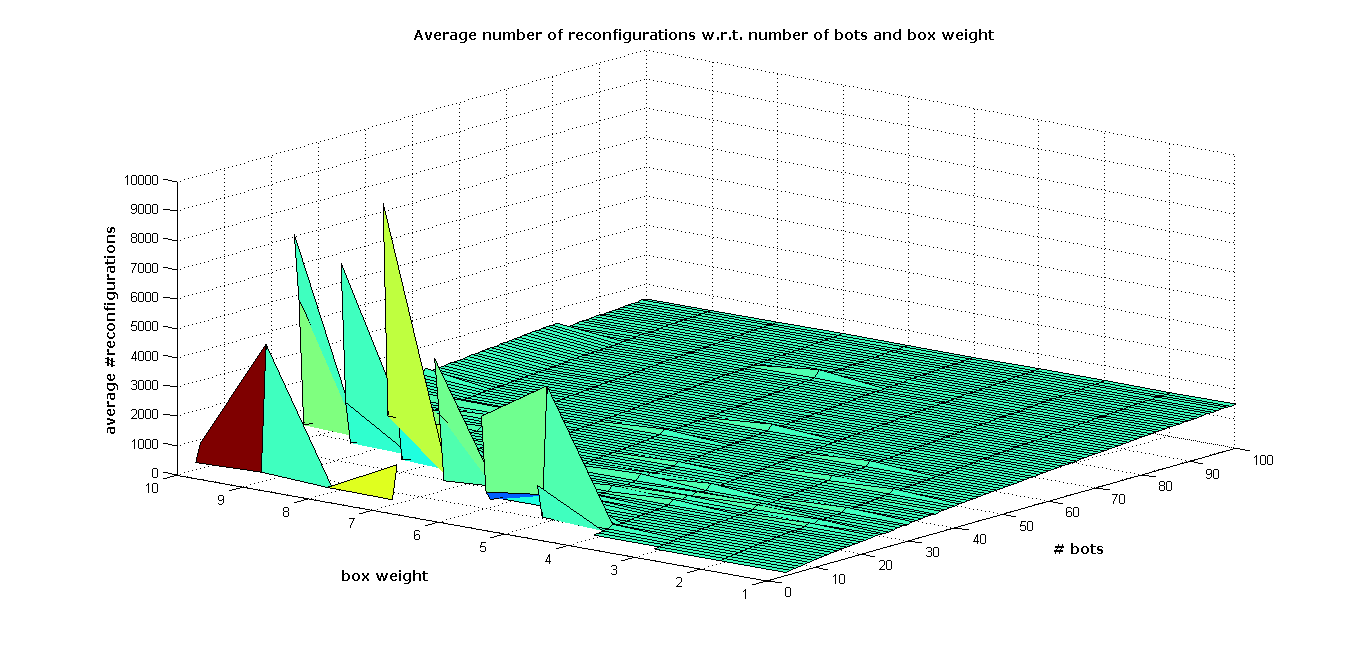
\includegraphics[scale=0.45]{images/bots_vs_weight}}
\caption{The variation of the number of bots required to solve a specific configuration. We used one box of various weights that need to be pushed over a gap. The results are averaged over the different gap sizes within the $[0, 10]$ interval.}
\label{fig:botsvsweight}
\end{figure}

